\newpage
\section*{先从训练与采样流程理解扩散模型}

先看扩散模型如何训练和采样。训练时，我们用已知的加噪规则，在任意指定的噪声水平下把干净样本变成带噪样本，再训练神经网络从带噪样本估计干净信号。生成时，从一个新抽取的噪声样本出发，每一步都用网络预测干净信号，同时逐步降低噪声水平。样本就在这个过程中逐渐呈现数据分布的结构。

\msgu{消息}{}{
创建多种噪声级别的噪声数据，学习预测干净的信号，并通过从高噪声到低噪声重复应用此预测来生成。
}
\paragraph{创建噪声数据。}

让我们准确地解释一下数据的噪声版本的实际含义。获取干净的数据样本
\[
\rvx_0\sim p_{\mathrm{data}},
\]
例如图像或我们关心的任何其他类型的数据。我们在噪声水平上破坏它 $t$ 通过混合独立高斯噪声\footnote{
公式
$\rvx_t=\alpha_t\rvx_0+\sigma_t\beps$
给出选定噪声水平下的累积扰动 $t$ 直接。在 DDPM 和 Score SDE 中，通过许多较小的连续步骤添加噪声也可以获得该级别的相同边缘分布；看到
\Cref{sec:ddpm} 和 \Cref{ch:score-sde}。在后面介绍的离散 DDPM 表示法中，这种累积扰动被写为
\[
\rvx_i
=
\bar{\alpha}_i\rvx_0
+
\sqrt{1-\bar{\alpha}_i^2}\,\beps.
\]
}:
\[
\rvx_t
=
\alpha_t\rvx_0+\sigma_t\beps,
\qquad
\beps\sim\mathcal{N}(\bm{0},\rmI).
\]
想想 $\alpha_t$ 和 $\sigma_t$ 作为两个旋钮，预先固定，用于设置在噪声级别有多少干净信号和多少噪声进入混音
$t$。最简单的选择， $\alpha_t=1$ 和 $\sigma_t=t$，给出
\[
\rvx_t=\rvx_0+t\beps.
\]
现在 $t$ 实际上是一个噪声旋钮：将其转向零并 $\rvx_t$ 接近干净样本；将其调大并添加噪声项 $t\beps$
越来越多地接管。

\begin{figure}[!ht]
\centering
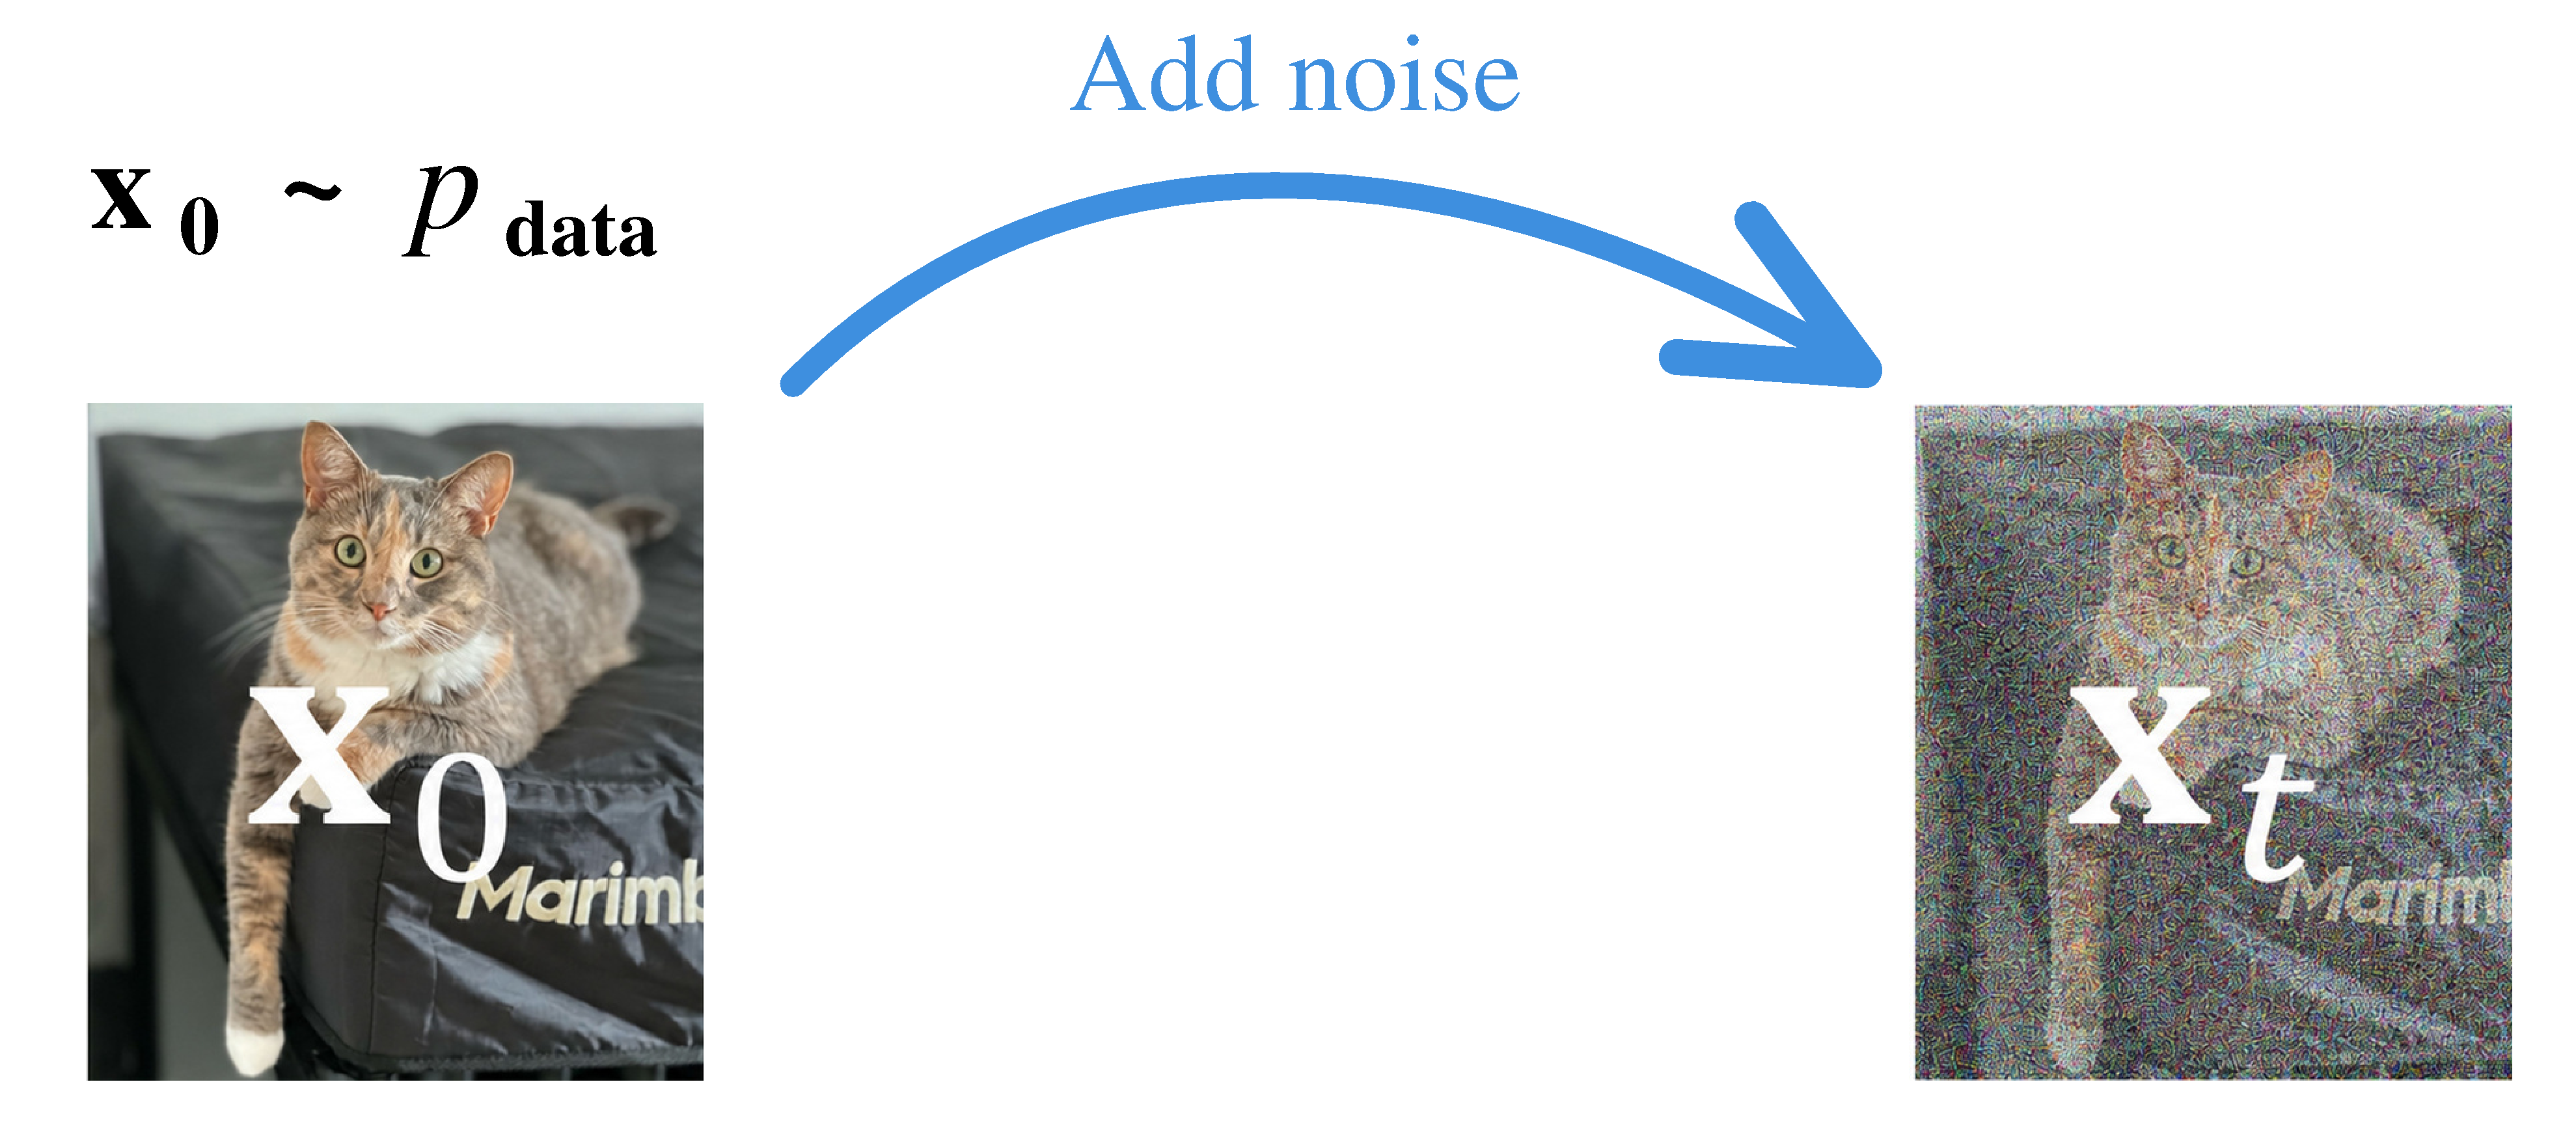
\includegraphics[width=0.6\linewidth]{Images/PartA/intro_forward.pdf}
\caption{\textbfs{前向扩散。} 干净的样本 $\mathbf{x}_0$ 已损坏并产生含噪观测结果 $\mathbf{x}_t$ 处于噪声水平 $t$.
\figcredit{由作者创建。}}
\label{fig:ill-forward}
\end{figure}

更一般地说，每个噪声水平 $t$ 定义分布 $p_t$ 噪声样本过多。想想很有用 $p_t$ 作为 \emph{快照}: 如果我们使用相同的值生成许多噪声样本 $t$，他们的分布是 $p_t$.选择计划 $(\alpha_t,\sigma_t)$ 以便这些快照移动
从干净的数据到简单的噪声分布：
\[
p_0=p_{\mathrm{data}}
\qquad\longrightarrow\qquad
p_t
\qquad\longrightarrow\qquad
p_T\approx p_{\mathrm{prior}},
\]
其中 $p_{\mathrm{prior}}$ 通常是高斯分布，很容易
从中取样。因此，这族分布
\[
\{p_t\}_{t\in[0,T]}
\]
描述分布如何随着噪声水平逐渐变化
增加。




\paragraph{训练：学习预测干净信号。}

现在有了一种破坏数据的方法，训练几乎变得
机械的，它取决于一个关键技巧：因为我们就是那个
破坏数据，我们总是知道正确的答案。构建一个单一的
训练示例，我们采样干净的数据 $\rvx_0$，选择噪声级别
$t$，拉动噪声 $\beps$，并形成
\[
\rvx_t
=
\alpha_t\rvx_0+\sigma_t\beps.
\]
我们自己制造了 $\rvx_t$，所以我们已经确切地知道哪个
清洁 $\rvx_0$ 生产它。

然而，网络永远不会直接看到 $\rvx_0$ 或 $\beps$。它看到
仅对 $(\rvx_t,t)$，损坏的观察以及如何损坏
是的。它的任务是猜测其背后的干净数据：
\[
\rvx_0^{\mathrm{pred}}
:=
\rvx_{\bphi}(\rvx_t,t).
\]
因为我们知道真正的目标，所以我们可以对这个猜测进行评分并改进它
使用普通的平方误差损失：
\[
\left\|
\rvx_0^{\mathrm{pred}}-\rvx_0
\right\|_2^2.
\]

\msgu{留言}{}{
简而言之：使用已知的干净目标创建含噪观测，隐藏
来自网络的目标，并训练它来预测目标。
}

对不同的数据样本反复抽取噪声、改变噪声强度，同一个网络就能在从轻微扰动到近乎纯噪声的各种情况下预测干净样本。

平方误差下，网络能给出的最优预测是条件期望
\[
\rvx_0^*(\rvx_t,t)
=
\E[\rvx_0|\rvx_t,t].
\]
不同的干净样本可能产生相似的含噪观测 $\rvx_t$。只要噪声强度非零，这种不确定性就会存在，且会随噪声增强而加剧。因此，网络学到的是对给定当前观测时所有可能的干净样本取条件平均\footnote{噪声强度由上下文明示时，通常简写为 $\E[\rvx_0|\rvx_t]$。}。

\paragraph{采样：从新抽取的噪声出发。}

训练后，网络能从含噪观测预测干净样本。生成新样本时，我们固定训练好的参数，记作 $\bphi^\times$，然后沿前向加噪的反方向从纯噪声出发。
\[
\tilde{\rvx}_T\sim p_{\mathrm{prior}}.
\]
我们在生成过程的状态 $\tilde{\rvx}_t$ 上加波浪号，以区别于训练期间前向加噪得到的 $\rvx_t$。

初始状态 $\tilde{\rvx}_T$ 直接从先验分布抽取，因此没有某个与它对应的真实样本 $\rvx_0$ 可供恢复。每到一个噪声水平，采样器都请训练好的网络估计当前状态对应的干净信号，再据此向数据分布迈进一步。具体来说，把当前状态 $\tilde{\rvx}_t$ 输入网络，得到对干净样本的预测
\[
\rvx_0^{\mathrm{pred}}
:=
\rvx_{\bphi^\times}(\tilde{\rvx}_t,t).
\]
对于 $t>0$，我们还可以计算隐含噪声残差，定义为从当前状态移除预测信号后剩下的任何内容：
\[
\beps_t^{\mathrm{pred}}
:=
\frac{
\tilde{\rvx}_t-\alpha_t\rvx_0^{\mathrm{pred}}
}{
\sigma_t
}.
\]
这两个量不是独立的猜测：通过构造，它们精确地重新组合了当前状态，
\[
\tilde{\rvx}_t
=
\alpha_t\rvx_0^{\mathrm{pred}}
+
\sigma_t\beps_t^{\mathrm{pred}}.
\]

这是单个采样步骤背后的想法：保持预测信号和预测噪声不变，但使用系数重新混合它们以获得略低的噪声水平 $t-\Delta t$ 代替
$t$:
\[
\tilde{\rvx}_{t-\Delta t}
=
\alpha_{t-\Delta t}\rvx_0^{\mathrm{pred}}
+
\sigma_{t-\Delta t}\beps_t^{\mathrm{pred}}.
\]
同样，这是在当前状态之上的一个小更新，
\begin{equation}\label{eq:ddpm-first-try}
\tilde{\rvx}_{t-\Delta t}
=
\tilde{\rvx}_t
+
(\alpha_{t-\Delta t}-\alpha_t)\rvx_0^{\mathrm{pred}}
+
(\sigma_{t-\Delta t}-\sigma_t)\beps_t^{\mathrm{pred}}.
\end{equation}

这是第一步。我们现在喂养新的状态 $\tilde{\rvx}_{t-\Delta t}$
回到网络，获取更新的、通常不同的干净数据预测，并进一步降低噪声。采样正是这个循环，从 $t=T$ 下降到 $t=0$.

\msgu{消息}{}{
简而言之：从新鲜噪声开始，预测干净的信号，逐步降低噪声水平，然后再次预测。
}

\begin{figure}[th!]
\vspace{-0.5cm}
\centering
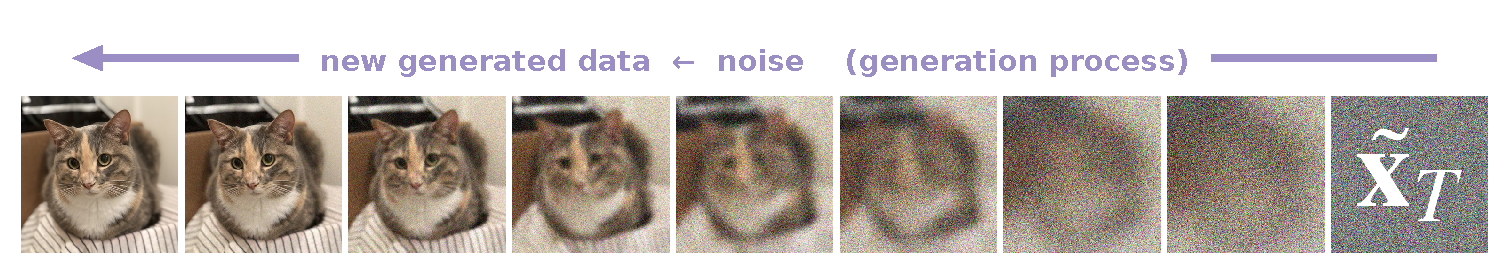
\includegraphics[width=\linewidth]{Images/PartA/intro-diffusion-reverse.pdf}
\caption{\textbfs{扩散生成。} 从新鲜噪声开始
$\tilde{\mathbf{x}}_T\sim p_{\mathrm{prior}}$随着噪声水平的降低，重复的模型预测会构建新的样本。
\figcredit{由作者创建。}}
\label{fig:ill-reverse}
\end{figure}

此时一个自然的问题：为什么不简单地输出第一个预测 $\rvx_0^{\mathrm{pred}}$ 然后停止？由于在高噪声水平下，当前状态携带的有关干净结构的信息非常少，因此预测只不过是许多合理样本的粗略平均值。转向稍微较低的噪声水平可以使网络的工作状态稍微不那么模糊，因此它的下一个预测可以变得更加清晰。如此重复多次，才能逐渐呈现出真正详细的样本\footnote{稍后我们将将此确定性更新连接到 DDIM 采样及其欧拉型解释~\citep{song2020denoising} 在 \Cref{sec:revisit-ddim};随机 DDPM 采样器的介绍 \Cref{sec:ddpm}.}.

\paragraph{一个简单的例子。}让我们使用之前运行的示例（其中 $\alpha_t=1$ 和 $\sigma_t=t$）来具体说明这一点。代入上面的更新给出
\[
\tilde{\rvx}_{t-\Delta t}
=
\rvx_0^{\mathrm{pred}}
+
(t-\Delta t)
\frac{
\tilde{\rvx}_t-\rvx_0^{\mathrm{pred}}
}{
t
},
\]
重新排列成简单的加权平均值，
\[
\tilde{\rvx}_{t-\Delta t}
=
\frac{t-\Delta t}{t}\tilde{\rvx}_t
+
\frac{\Delta t}{t}\rvx_0^{\mathrm{pred}}.
\]
当 $\Delta t$ 较小时，下一状态就是当前状态与网络预测的干净样本的加权平均。

每一步都把样本向网络\emph{当前}预测的干净样本推进一点。走到噪声更少的新状态后，网络通常会给出不同的预测。最终样本由一连串逐步更新的预测共同决定。

\paragraph{ 这如何连接到后续章节？}

这里用干净数据预测说明了扩散模型的基本流程。全书都会沿用这一思路。训练时，从干净数据构造带噪样本，再学习如何从中预测有用的信息。生成时，从新抽取的噪声出发，用训练得到的预测逐步降低噪声水平，构造新样本。

以下章节从不同的数学角度解释了相同的过程
观点。 \Cref{ch:variational} 将 DDPM 连接到潜变量模型，
其中固定噪声过程扮演编码器的角色，学习到的
反向转换起到解码器的作用。
\Cref{ch:score-based}描述了通过分数去噪，它提供了
更新噪声样本的方向。
\Cref{ch:score-sde} 从离散噪声水平转向连续时间和
描述了通过逆时随机动力学产生的过程。
\Cref{ch:flow-based} 相反，将生成视为沿着
从简单先验到数据分布的连续路径。
最后，\Cref{ch:all-equivalent} 解释了这些观点是如何联系起来的。

主要要点很简单：扩散模型从噪声版本中学习
许多噪声水平的数据，并且生成使用这些学习的预测
反复将新的噪声转化为新的样本。
